$X_{26}$ is the Circumcenter of the Tangential Triangle \cite{mw}. Its sides are tangent to the Circumcircle at the vertices. If the 3-periodic is a right-triangle, its hypotenuse is a diameter of the Circumcircle, and $X_{26}$ is unbounded.

We saw above that:

\begin{itemize}
\item $a/b<\alpha_4$, the 3-periodic family is all-acute, i.e., the locus of $X_{26}$ is compact. Figure~\ref{fig:orthocenter_loci} (top left).
\item $a/b=\alpha_4$, the family is all-acute except when one of its vertices coincides with the top or bottom vertex of the EB, Figure~\ref{fig:orthocenter_loci} (bottom left). In this case the 3-periodic is a right triangle and $X_{26}$ is unbounded.
\item $a/b>\alpha_4$, the family features both acute and obtuse triangles. The transition occurs at for four right-angle 3-periodics whose $X_4$ is on the EB, Figure~\ref{fig:orthic_incenter_locus}(b). Here too $X_{26}$ flies off to infinity, Figure~\ref{fig:x26}.
\end{itemize}

\begin{figure}
    \centering
    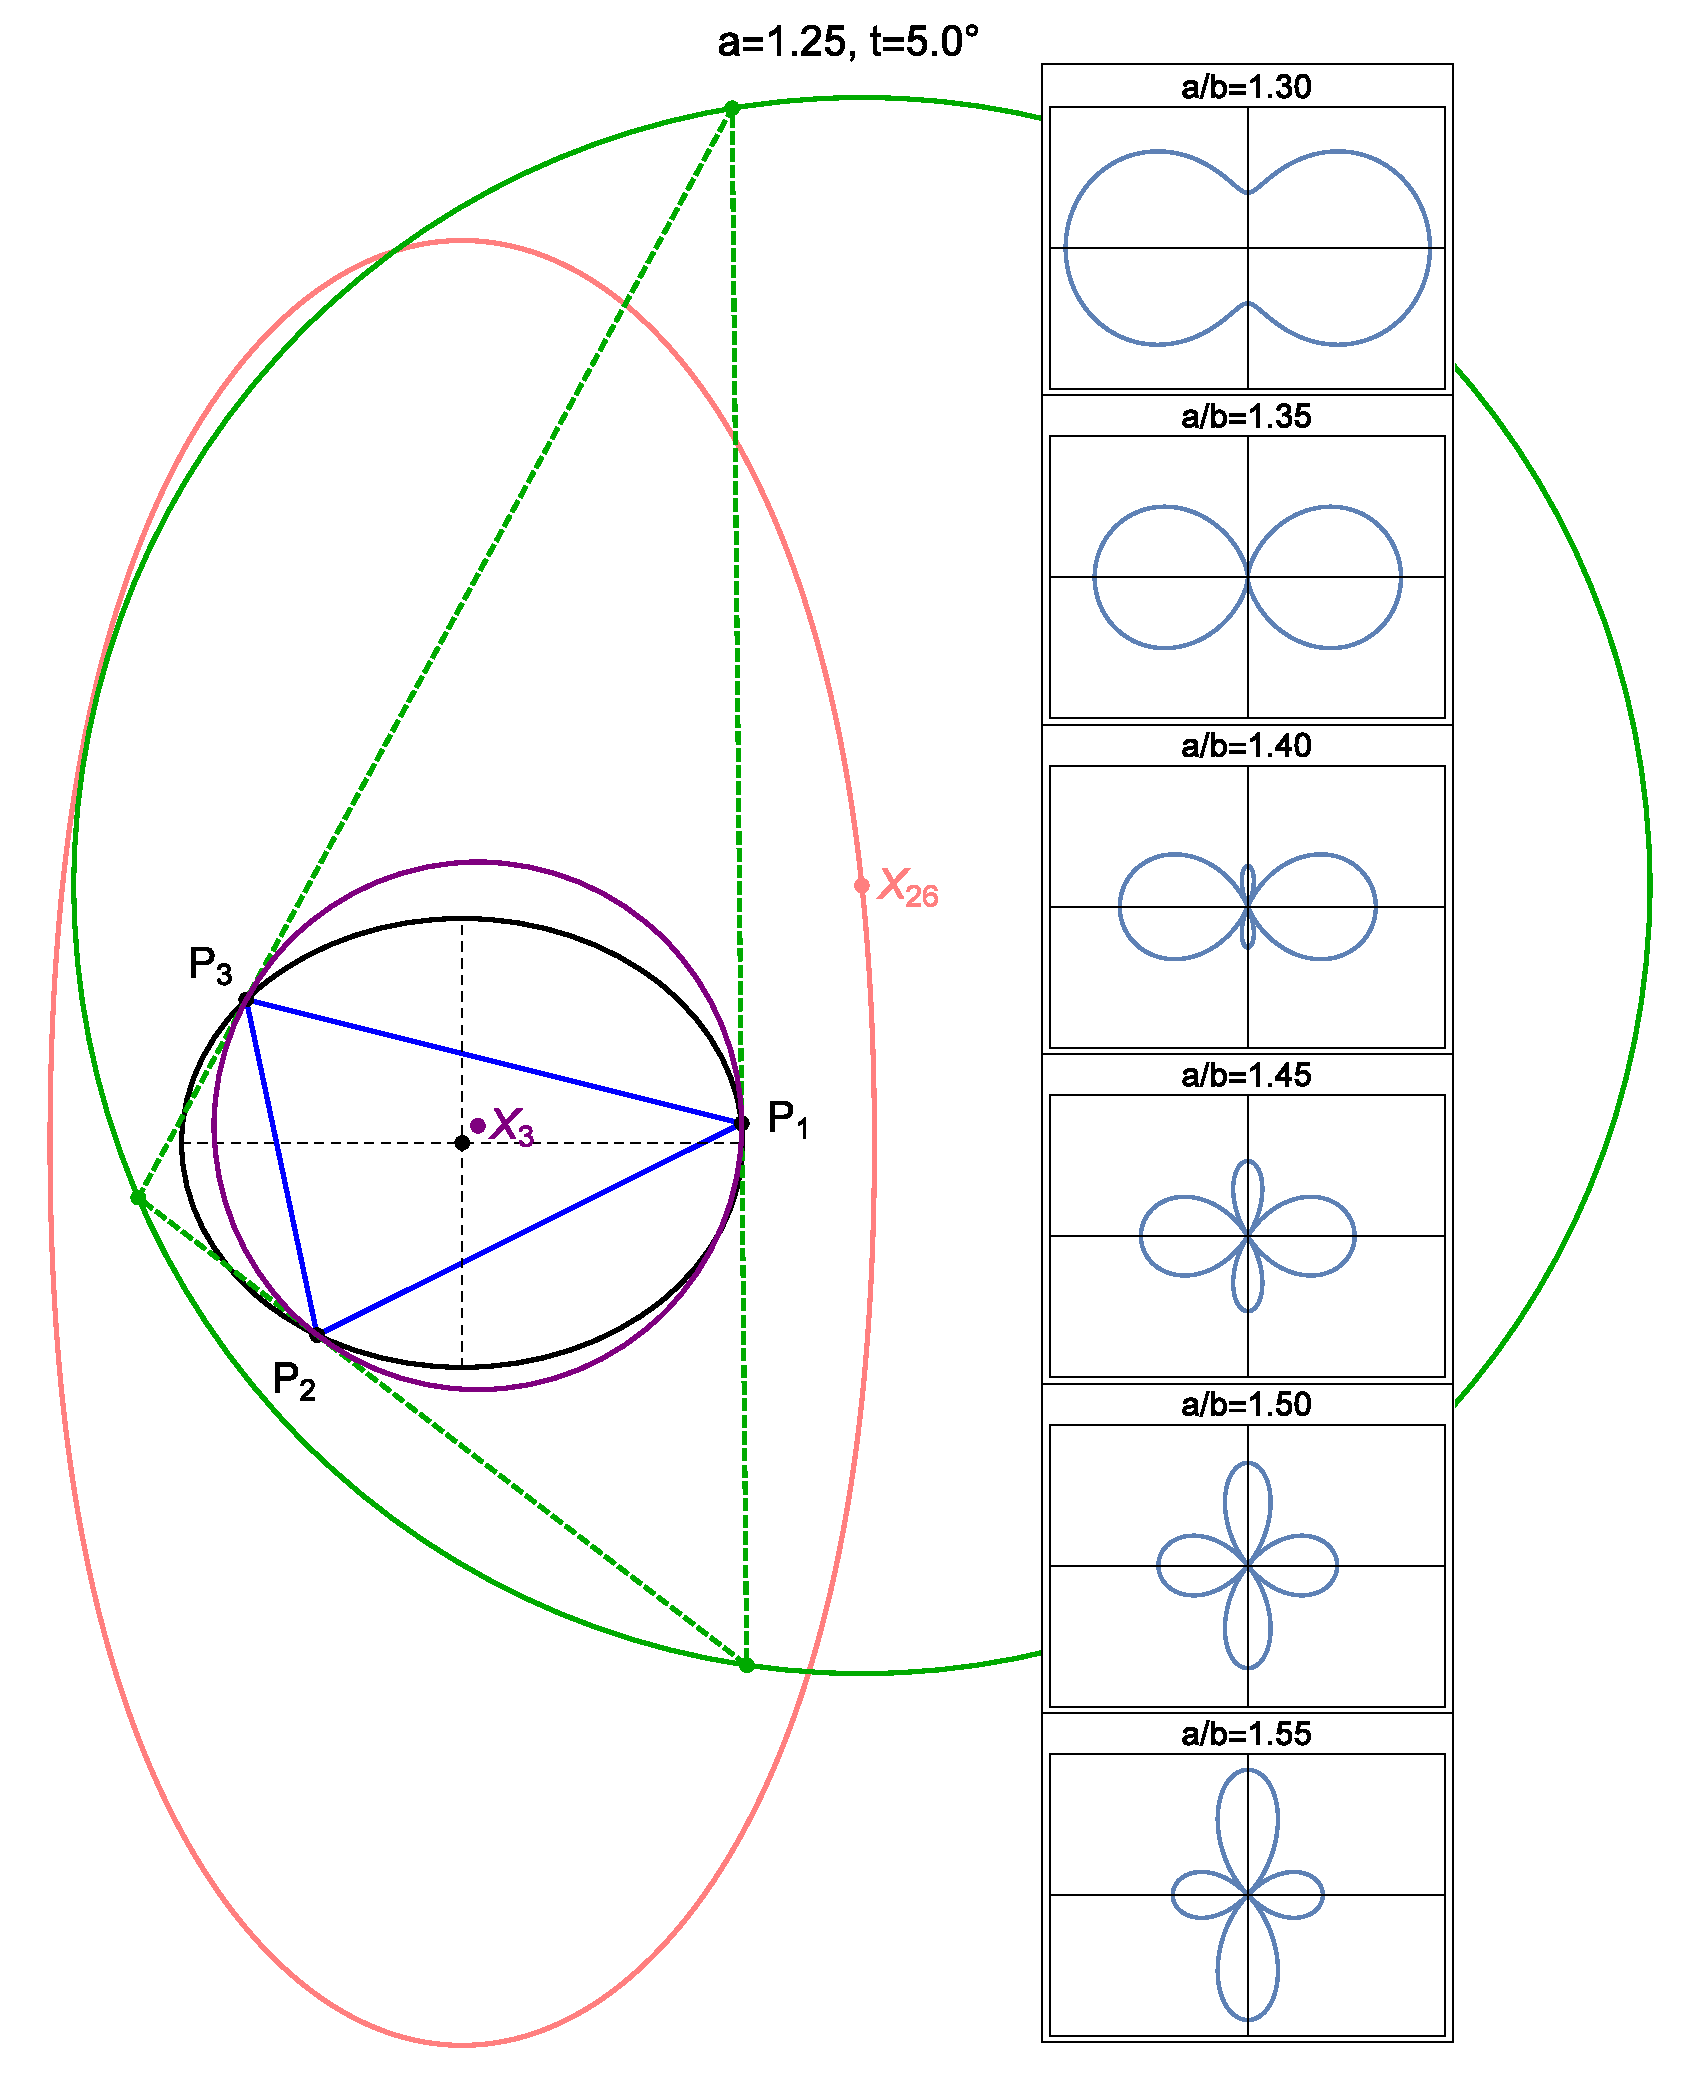
\includegraphics[width=.8\textwidth]{pics/1060_x26.eps}
    \caption{The locus of $X_{26}$ for a 3-periodic (blue) in an $a/b=1.25$ EB (black). Also shown is the 3-periodic's Circumcircle (purple) and its Tangential Triangle \cite{mw} (dashed green). $X_{26}$ is the center of the latter's Circumcircle (solid green). Its locus is non-elliptic. In fact, when $a/b{\geq}\alpha_4$, the 3-periodic family will contain right-triangles ($X_4$ crosses the EB). At these events, $X_{26}$ flies off to infinity. The right inset shows an inversion of $X_{26}$  with respect to the EB center for various values of $a/b$. When $a/b>\alpha_4$, the inversion goes through the origin, i.e., $X_{26}$ is at infinity.}
    \label{fig:x26}
\end{figure}

